% Staging document: ONLY supplementary material following the original manuscript's \appendix.
% Release subject to verifying paper-specific public assets; no private repository data included.
\documentclass[11pt]{article}
\usepackage[margin=1in]{geometry}
\usepackage{amsmath,amssymb,booktabs,longtable,array,graphicx,float,flafter,placeins,microtype}
\usepackage[hidelinks]{hyperref}
\graphicspath{{../figures/}{figures/}}
\title{Supplementary Evidence\\[0.3em]\large An Overlapping Local Relational Geometry of Early Mouse Embryogenesis}
\author{Zed James}
\date{October 2026}
\begin{document}
\maketitle
\appendix

\section{Supplementary complete lane construction}

\begin{longtable}{@{}llrrrr@{}}
\caption{Complete nine-lane construction: all 27 pair-symmetric q50 thresholds, edge counts, and endpoint counts.}
\label{tab:supp_laneauthority}\\
\toprule
Lane & Pair & Genes & \(\epsilon\) & Edges & Source/target endpoints\\
\midrule
\endfirsthead
\toprule
Lane & Pair & Genes & \(\epsilon\) & Edges & Source/target endpoints\\
\midrule
\endhead
$\ell_0$&P12&14660&0.443926&4798&656/509\\
$\ell_0$&P13&14660&0.413115&4355&572/631\\
$\ell_0$&P23&14660&0.447197&4959&545/791\\
$\ell_1$&P12&14660&0.411419&4325&648/517\\
$\ell_1$&P13&14660&0.381856&3762&544/659\\
$\ell_1$&P23&14660&0.412007&3657&545/791\\
$\ell_2$&P12&14660&0.364210&4655&642/523\\
$\ell_2$&P13&14660&0.335290&4244&541/662\\
$\ell_2$&P23&14660&0.365148&4443&534/802\\
$\ell_3$&P12&14660&0.375291&4605&629/536\\
$\ell_3$&P13&14660&0.349995&3760&566/637\\
$\ell_3$&P23&14660&0.375740&4453&552/784\\
$\ell_4$&P12&14660&0.381581&4930&633/532\\
$\ell_4$&P13&14660&0.354196&4369&566/637\\
$\ell_4$&P23&14660&0.383836&5304&548/788\\
$\ell_5$&P12&10300&0.430363&5200&656/509\\
$\ell_5$&P13&10300&0.402765&4559&575/628\\
$\ell_5$&P23&10300&0.434458&5411&522/814\\
$\ell_6$&P12&10307&0.441695&4880&634/531\\
$\ell_6$&P13&10307&0.408974&4533&537/666\\
$\ell_6$&P23&10307&0.440862&4692&531/805\\
$\ell_7$&P12&10268&0.439892&4708&656/509\\
$\ell_7$&P13&10268&0.412815&4559&584/619\\
$\ell_7$&P23&10268&0.445180&5051&537/799\\
$\ell_8$&P12&10207&0.442949&4516&646/519\\
$\ell_8$&P13&10207&0.413301&4951&576/627\\
$\ell_8$&P23&10207&0.448554&5185&550/786\\
\bottomrule
\end{longtable}

\section{Supplementary lane-vote anatomy}

\begin{figure}[H]
\centering
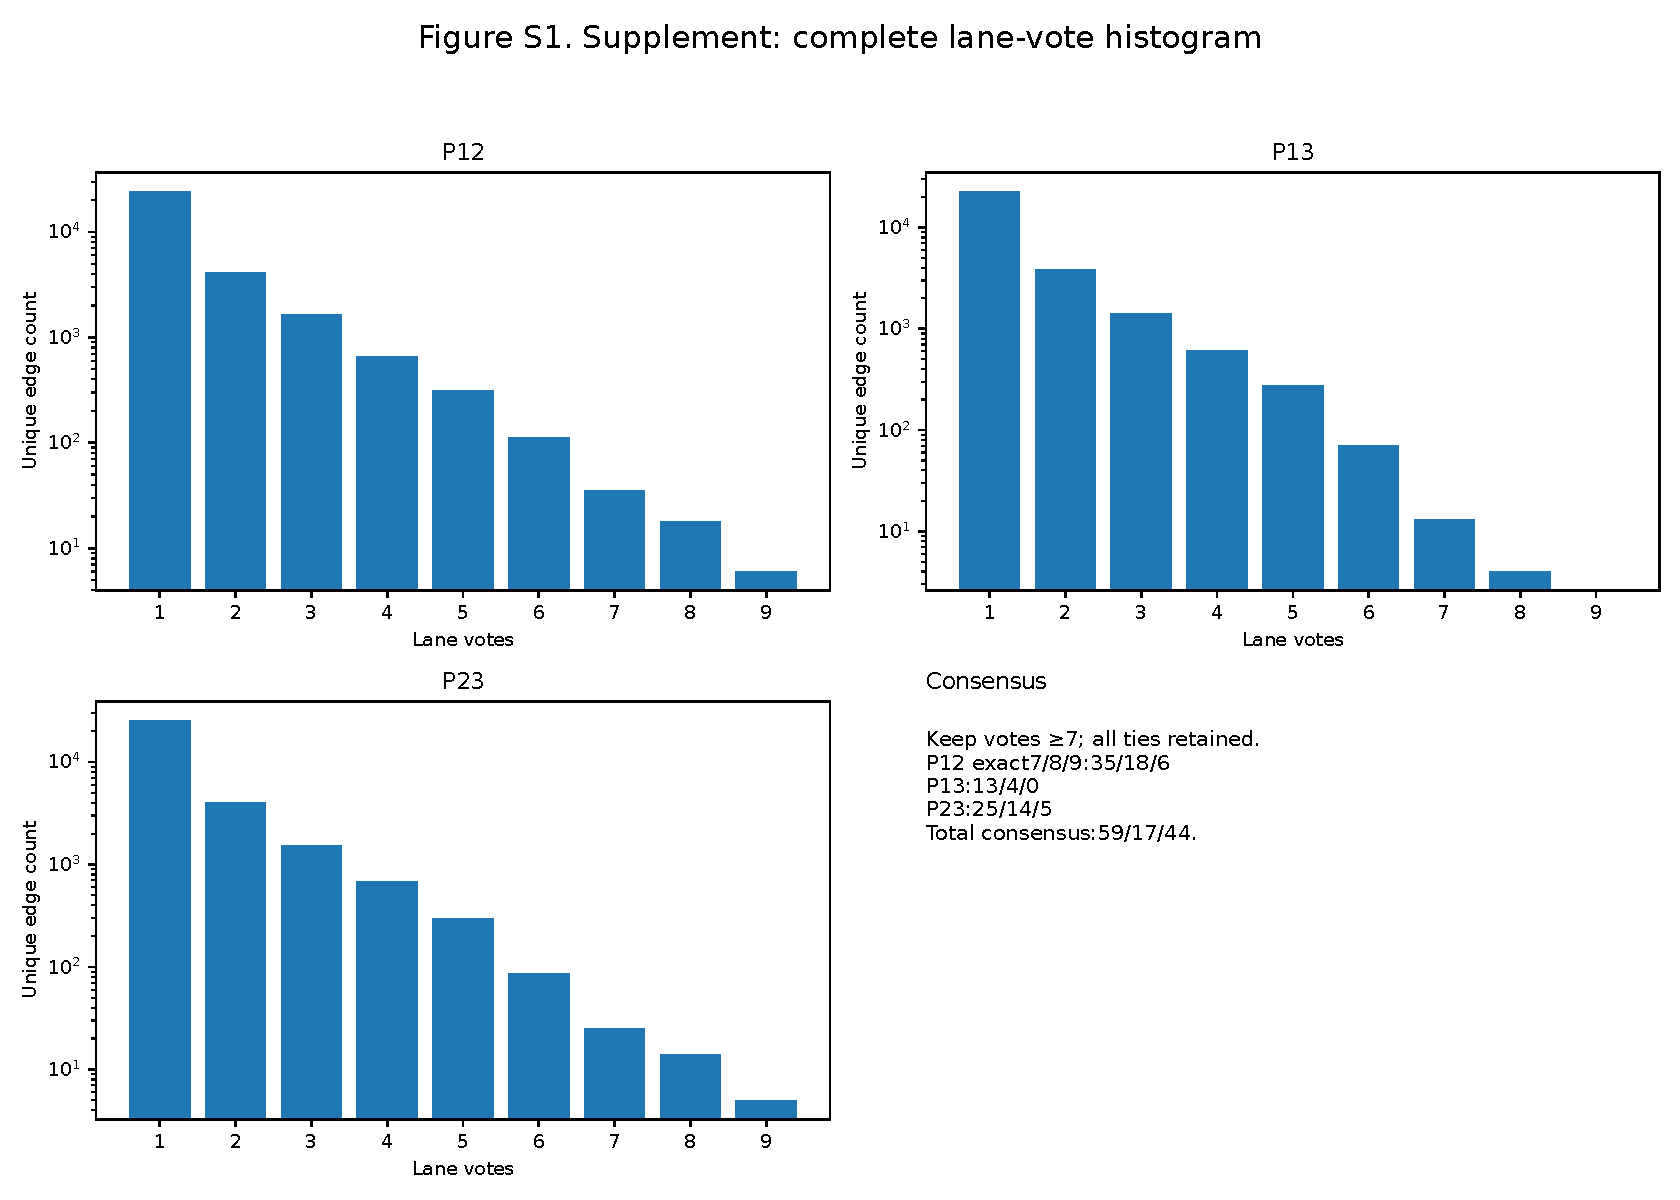
\includegraphics[width=0.85\textwidth]{RMMO_Paper3_FigureS1_ConsensusVoteHistogram.pdf}
\caption{Complete candidate-edge vote histogram. The vertical line marks the seven-vote consensus threshold.}
\end{figure}
\FloatBarrier

\section{Supplementary retention trajectory}

\begin{figure}[H]
\centering
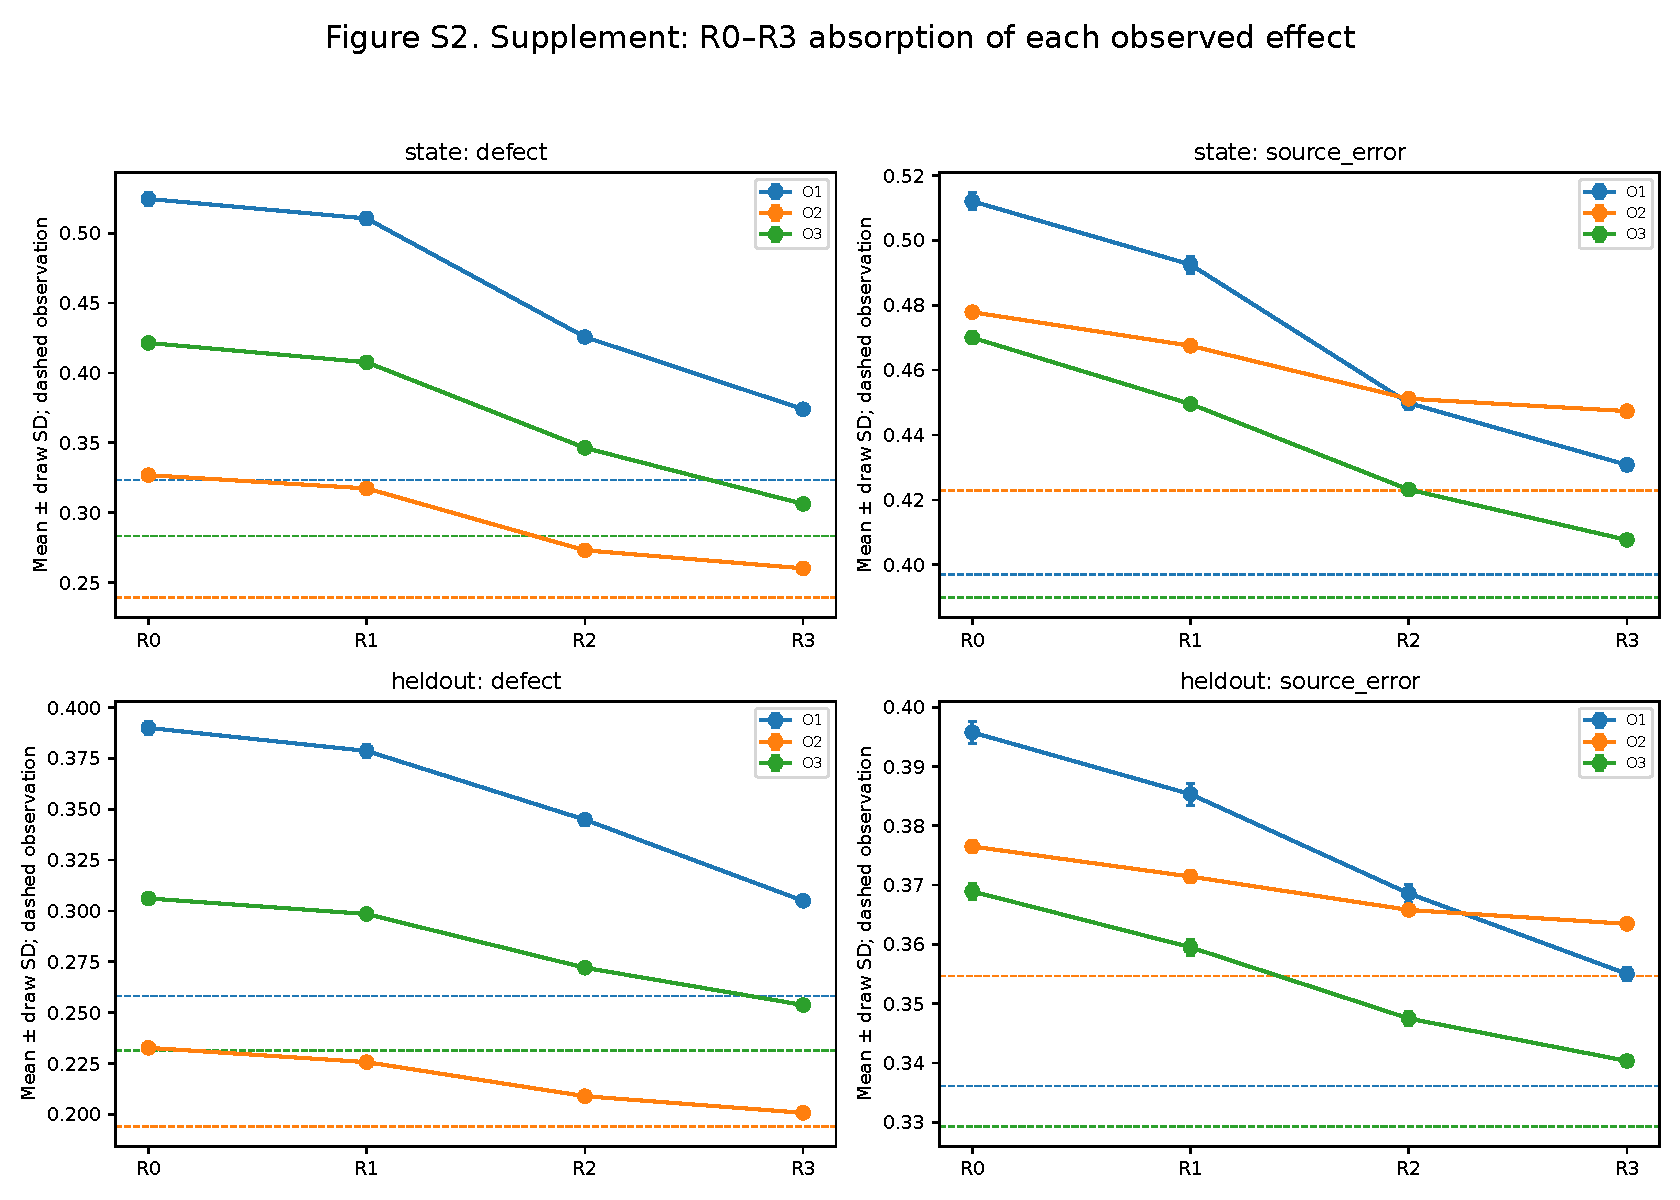
\includegraphics[width=0.85\textwidth]{RMMO_Paper3_FigureS2_RetentionTrajectories.pdf}
\caption{Selected q25 null means for O1 across \(R0\) (size only) through \(R3\) (+ endpoint support). Full 48-component surfaces, SDs, standardized separations, and family statistics are included in the companion.}
\end{figure}
\FloatBarrier


\section{Supplementary domain-scale sensitivity}
\label{app:scales}
\begin{figure}[H]
\centering
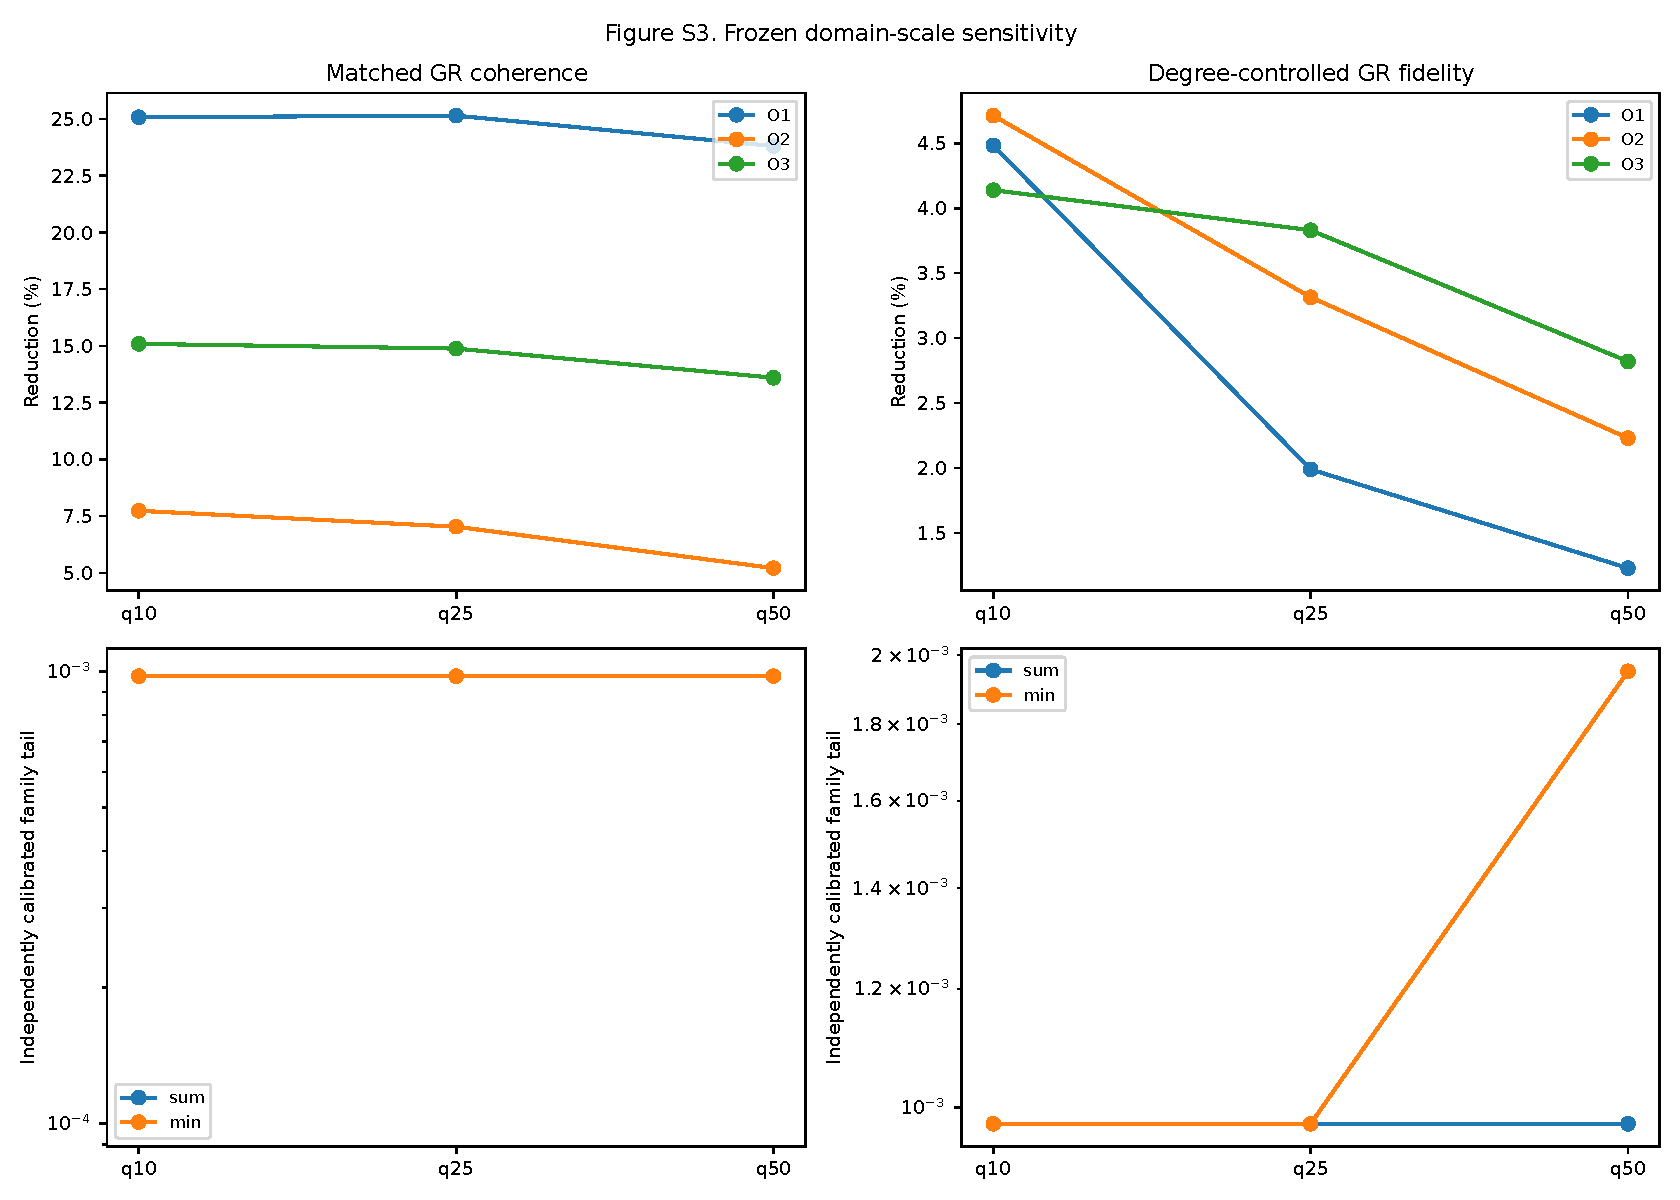
\includegraphics[width=0.86\textwidth]{RMMO_Paper3_FigureS3_DomainScaleSensitivity.pdf}
\caption{Frozen q10/q25/q50 sensitivity of the two principal \(G_R\) relational effects under the final independent-calibration convention. Matched-target coherence remains positive in O1--O3 at every scale. Degree-controlled source fidelity also retains positive component directions, while O1 remains individually unsupported after maxT adjustment.}
\label{fig:scales}
\end{figure}
\FloatBarrier


\section{Supplementary inferential calibration closure}

Independent same-model calibration banks fix the standardization used by every manuscript-facing maxT, \(T_\Sigma\), and \(T_{\min}\) statistic, while the original inferential draws supply their empirical ranks. Across all reported analyses, 108/108 component maxT decisions and 72/72 aggregate/minimum decisions are preserved at \(\alpha=0.05\). The primary held-out degree-controlled O1 maxT tail is 0.122927 under the final convention; the q10 and q50 values are 0.060488 and 0.139512. Complete component- and test-level calibration results are provided in the reproducibility package.

\section{Supplementary retained-structure effect surface}
\label{app:retention_surface}
\begin{figure}[H]
\centering
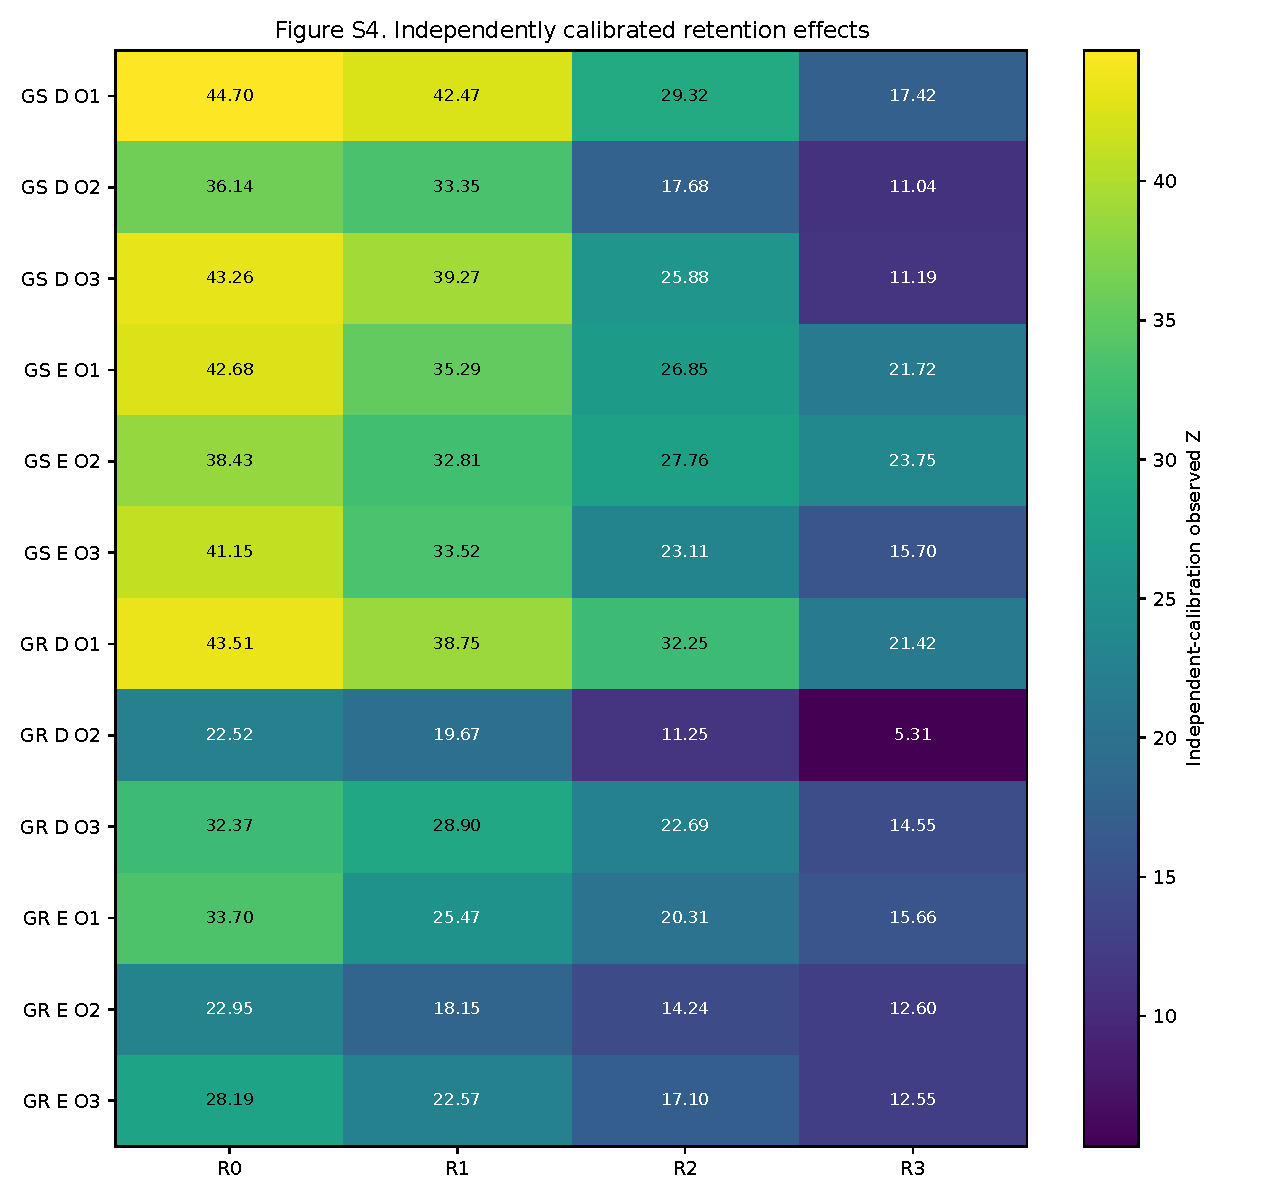
\includegraphics[width=0.94\textwidth]{RMMO_Paper3_FigureS4_RetentionEffectSurface.pdf}
\caption{Complete independently calibrated standardized-separation surface for the four retained-structure references, from \(R0\) (size only) through \(R3\) (+ endpoint support). Rows contain state and \(G_R\) defect/source-error statistics for O1--O3; columns show progressively richer retained structure. The calibration constants are fixed independently; the inferential banks remain frozen.}
\label{fig:retention_heatmap}
\end{figure}
\FloatBarrier

\section{Final finite global-boundary tables}

\begin{table}[htbp]
\centering
\small
\caption{Exact q25 composition counts.}
\begin{tabular}{@{}lrrrrrr@{}}
\toprule
Route & Direct & Composed & Common & Direct only & Composed only & Equal\\
\midrule
\(1\to2\to3\)&329&4161&250&79&3911&No\\
\(1\to3\to2\)&517&1677&371&146&1306&No\\
\(2\to1\to3\)&2105&862&321&1784&541&No\\
\bottomrule
\end{tabular}
\end{table}

\begin{table}[htbp]
\centering
\small
\caption{Historical existential bridge criterion on strict q25 overlaps.}
\begin{tabular}{@{}lrrrrr@{}}
\toprule
Overlap & Tested & Bridge present & Failing & Fraction & Complete\\
\midrule
O1&207&165&42&0.797&No\\
O2&287&168&119&0.585&No\\
O3&252&186&66&0.738&No\\
\bottomrule
\end{tabular}
\end{table}

\end{document}
